%% This is an example first chapter.  You should put chapter/appendix that you
%% write into a separate file, and add a line \include{yourfilename} to
%% main.tex, where `yourfilename.tex' is the name of the chapter/appendix file.
%% You can process specific files by typing their names in at the 
%% \files=
%% prompt when you run the file main.tex through LaTeX.
\chapter{Introduction}\label{intro-ch}

\section{Distributed Systems}


With the rise of big data, new data processing systems have been designed to help process it. 
Instead of relying on using just onemore powerful computers, these systems use many computers and are thus distributed in nature due to economic costs,scalability, and fault tolerance. Because programming in these  distributed environments is challenging, data processing systems
try to abstract this from the user and provide a simple interface for them. One of the most popular systems is Map Reduce,
invented by Google, which provides a simple map and reduce operation to the user. Another of these systems is Spark, which provides
a slightly more expressive api then map reduce and also has different modes of fault tolerance than spark along with caching. 
One key and slow stage that both of these systems have, is that because they are distributed in nature, they have a stage
where data must be transferred between machines, called the shuffle stage. This shuffle stage can be the bottleneck and be the reason for low performance of jobs.
\section{Shuffle} 

\subsection{Shuffle Introduction}
In map reduce, data is loaded onto different computers and an computation is performed on it (the map phase) that results 
in a group of key value pairs. The final phase of map reduce,the reduce phase assumes that all key-value pairs with the same
key are grouped onto the same machine. Thus, an intermediate phase that these systems handle themselves is the shuffle phase where
data is transferred so that all key value pairs with the same keys result to be on the same machine. 
\\

The following example in Figure~\ref{fig:shuffle_basic} details the inner workings 
of what happens in a shuffle for map reducer. Suppose we want to count the 
number of letters in a distributed file. The mappers will count the number of
letters in their individual file. However, we need to aggregate this and 
thus all the counts for letter a will be sent to worker1, letter b will be sent to worker 2,
letter c will be sent to worker c. These reducers will then promptly aggregate the counts that they receive from the 
mappers.

\begin{figure}[h]
\begin{center}
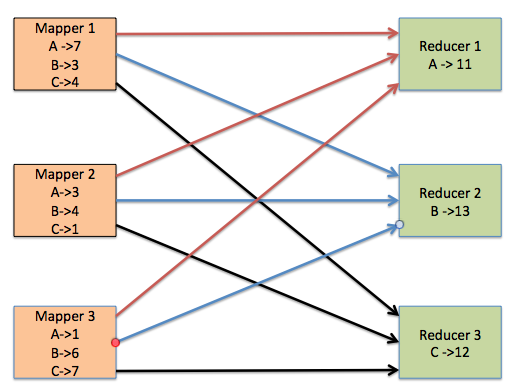
\includegraphics[scale=1.0]{./img/shuffle_basic.png}
\caption{Shuffle for Letter Count in Map Reduce}
\label{fig:shuffle_basic}
\end{center}
\end{figure}

Because of the huge amounts of keys, these systems do not deal with on the granurality of keys.
nstead, they deal with the concepts of partitions. These systems have different partitioning functions
that map key-value pairs to different partitions. Some popular partition schemes include range and hash partitioning.
As long as all the mappers agree to partition their data in the same way and send each partition that is the same to the same reducer, we are ensured that any two keys that are the same will be in the same partition. 

\subsection {Shuffle Analysis}

Throughout the shuffle process, we want to balance the amount of data being sent to the reducers. 
These systems are constrained by the slowest worker, so generally we want to minimize the latencies of the slowest worker.
By balancing the data being sent, we can first reduce the latency for network transfer. Second, because the data each node 
has to process is more balanced, we can reduce the execution time for the slowest node. We illustrate this in the following situation.
In Figure~\ref{fig:shuffle_unbalanced}, we demonstrate a common scenario that happens in these shuffle scenarios. Let us say we have a simple
partitioning scheme, where the reducer a partition lands up is determined by partition id mod the number of works. This seems reasonable
as typically we do not have extra information about the size of the partitions. This leads to situations where we one reducer receiving
50MB of data while another reducer gets 90MB of data. However, if we knew the size of each partition after the mappers have run,
we could more intelligently partition the data. As seen in Figure~\ref{fig:shuffle_balanced}, we see that by intelligently distributing the partitions in the same situation we can lead to each partition for 60MB. 


 \begin{figure}[h]
\begin{center}
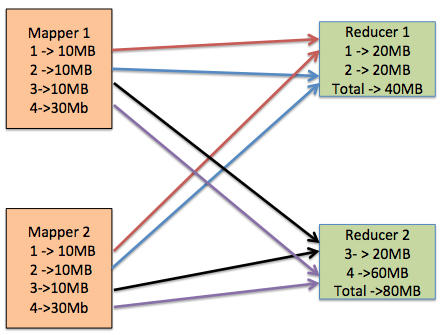
\includegraphics[scale=1.0]{./img/shuffle_unbalanced.png}
\caption{Unbalanced shuffle of partitions} 
\label{fig:shuffle_unbalanced.png}
\end{center}
\end{figure}

 \begin{figure}[h]
\begin{center}
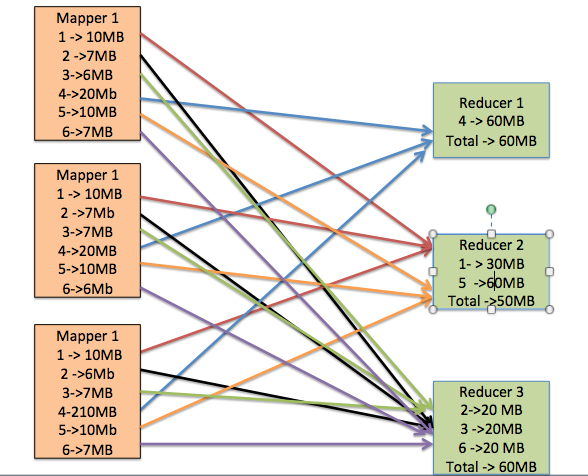
\includegraphics[scale=1.0]{./img/shuffle_balanced.png}
\caption{Balanced shuffle of partitions.}
\label{fig:shuffle_balanced.png}
\end{center}
\end{figure}

\section{Adaptive Scheduling of Joins}\label{intro-ch:eeg-overview}
The

